\chapter{State of the Art}
\label{state_of_art}
\linenumbers

\lettrine[lines=2]{I}{n traditional IT}, an attacker aims to understand the behavior of a program through various techniques so as to bring attacks aimed at changing its execution flow, functionalities or bypassing limits imposed by the licensing of such software. These attack techniques include a \textbf{preliminary study} of the program: a \textit{static analysis} (i.e., a preliminary analysis of the software without it running) and a \textit{dynamic analysis} (i.e., an analysis performed with the program running).\\
The result of these two preliminary investigation techniques is a \textbf{reverse engineering} of the software, which is useful for identifying any weaknesses or bugs and therefore planning an attack.

\bigskip
In the OT context, however, the concept of \textit{reverse engineering} is also associated with that of \textit{\textbf{process comprehension}}, a term coined by Green et al.'s \cite{green_et_al} to describe the understanding of the characteristics of the system and the physical elements of within it, that are responsible for its proper functioning.

\bigskip
Not much knowledge exists in the literature regarding the collection and analysis of information concerning the understanding and operation of an ICS: in Section \ref{sec:related_work} we will look at a quick overview of some of the existing literature on the subject and in the following sections we will focus in particular on one of the papers exposed.

\vfill

\section{Literature on Process Comprehension}
\label{sec:related_work}
\begin{description}
	\item[\textit{Keliris and Maniatikos}] The first approach presented in this section is by Keliris and Maniatakos \cite{keliris_maniatakos}: they present a methodology for automating the reverse engineering of ICS binaries based on a \textit{modular framework} (called ICSREF) that can reverse binaries compiled with CODESYS, one of the most popular and widely used PLC compilers, irrespective of the language used.
	
	\item[\textit{Yuan et al.}] Yuan et al. \cite{yuan_et_al} propose a \textit{data-driven} approach to discovering cyber-physical systems from data directly: to achieve this goal, they have implemented a framework whose purpose is to identify physical systems and transition logic inference, and to seek to understand the mechanisms underlying these cyber-physical systems, making furthermore predictions concerning their state trajectories based on the discovered models.
	
	\item[\textit{Feng et al.}] Feng et al. \cite{feng_swat} developed a framework that can generate system \textit{invariant rules} based on machine learning and data mining techniques from ICS operational data log. These invariants are then selected by systems engineers to derive IDS systems from them.
	
	The experiment results on two different testbeds, the \textit{Water Distribution system} (WaDi) and the \textit{Secure Water Treatment system} (SWaT), both located at the iTrust - Center for Research in Cyber Security at the University of Singapore \cite{itrust_site}, show that under the same false positive rate invariant-based IDSs have a higher efficiency in detecting anomalies than IDS systems based on a residual error-based model. 
	
	\item[\textit{Pal et al.}] Pal et al. \cite{pal_et_al} work is somewhat related to Feng et al.'s: this paper describes a data-driven approach to identifying invariants automatically using \textit{association rules mining} \cite{association_rules_mining} with the aim of generate invariants sometimes hidden from the design layout. The study has the same objective of Feng et al.'s and uses too the iTrust SwaT System as testbed.
	
	Currently this technique is limited to only pair wise sensors and actuators: for more accurate invariants generation, the technique adopted must be capable of deriving valid constrains across multiple sensors and actuators.
	
	\item[\textit{Winnicki et al.}] Winnicki et al. \cite{winnicki_et_al} instead propose a different approach to process comprehension based on the \textbf{attacker's perspective} and not limited to mere \textit{Denial of Service} (DoS): their approach is to discover the dynamic behavior of the system, in a semi-automated and process-aware way, through \textit{probing}, that is, slightly perturbing the cyber physical system and observing how it reacts to changes and how it returns to its original state. The difficulty and challenge for the attacker is to perturb the system in such a way as to achieve an observable change, but at the same time avoid this change being seen as a system anomaly by the IDSs.
	
	\item[\textit{Green et al.}] Green et al. \cite{green_et_al} also adopt an approach based on the attacker's perspective: this approach consists of two practical examples in a \textit{Man in the Middle} (MitM) scenario to obtain, correlate, and understand all the types of information an attacker might need to plan an attack to alter the process while avoiding detection.
	
	The paper shows \textit{step-by-step} how to perform a ICS \textbf{reconnaissance}, which is fundamental to process comprenension and thus to the execution of MiTM attacks.
	
	\item[\textit{Ceccato et al.}] Ceccato et al. \cite{ceccato} propose a methodology based on a \textit{black box dynamic analysis} of an ICS using a reverse engineering tool to derive from the scans performed on the memory registers of the exposed PLCs and network scans an approximate model of the physical process. This model is obtained by inferring statistical properties, business process and system invariants from data logs.
	
	The proposed methodology was tested on a non-trivial case study, using a testbed inspired by an industrial water treatment plant.
	
	In the next section I will examine this latest work in more detail, which will be the basis for my work and thus the subsequent chapters of this thesis.

\end{description}

\section{Ceccato et al.’s methodology for analyzing water-tank systems}
\label{sec:ceccato_metodology}
As mentioned earlier, the paper proposes a methodology based on a black box dynamic analysis of an ICS by identifying potential PLCs on the network and scanning the memory registers of the identified controllers to obtain an approximate model of the controlled physical process.

\bigskip
The first objective of this black box analysis is to associate the various memory registers of the target PLCs with a correspondence to the basic concepts of an ICS such as sensors (otherwise known as measurements), actuators, setpoints (range of values of a physical variable), network communications, and so on.\\
This is performed by analyzing the different types of memory registers associated with the Modbus protocol and trying to figure out what type of data they may contain.

The second objective is to put in relation the runtime evolution of these basic concepts.

\bigskip
To achieve this, Ceccato et al. developed a prototype tool \cite{plc_re} that performs reverse engineering of the physical system through four phases:

\begin{enumerate}
	\item \textbf{scanning of the system and data pre-processing}: data gathering is performed to generate the data logs of PLCs registers
	
	\item \textbf{graphs and statistical analysis}: provides information about the memory registers using graphs and statistical data derived from the gathered data
	
	\item \textbf{invariant inference and analysis}: generates system invariants and allows user to view invariants related to a given sensor or actuator
	
	\item \textbf{business process mining and analysis}: reconstructs, from event logs, the business process that shows how process is carried out
\end{enumerate}

In Figure \ref{fig:ceccato_overview} we have a schematic representation of the workflow related to this work. We will cover all these phases in detail in the next sections of this chapter. 

\begin{figure}[ht]
	\centering
	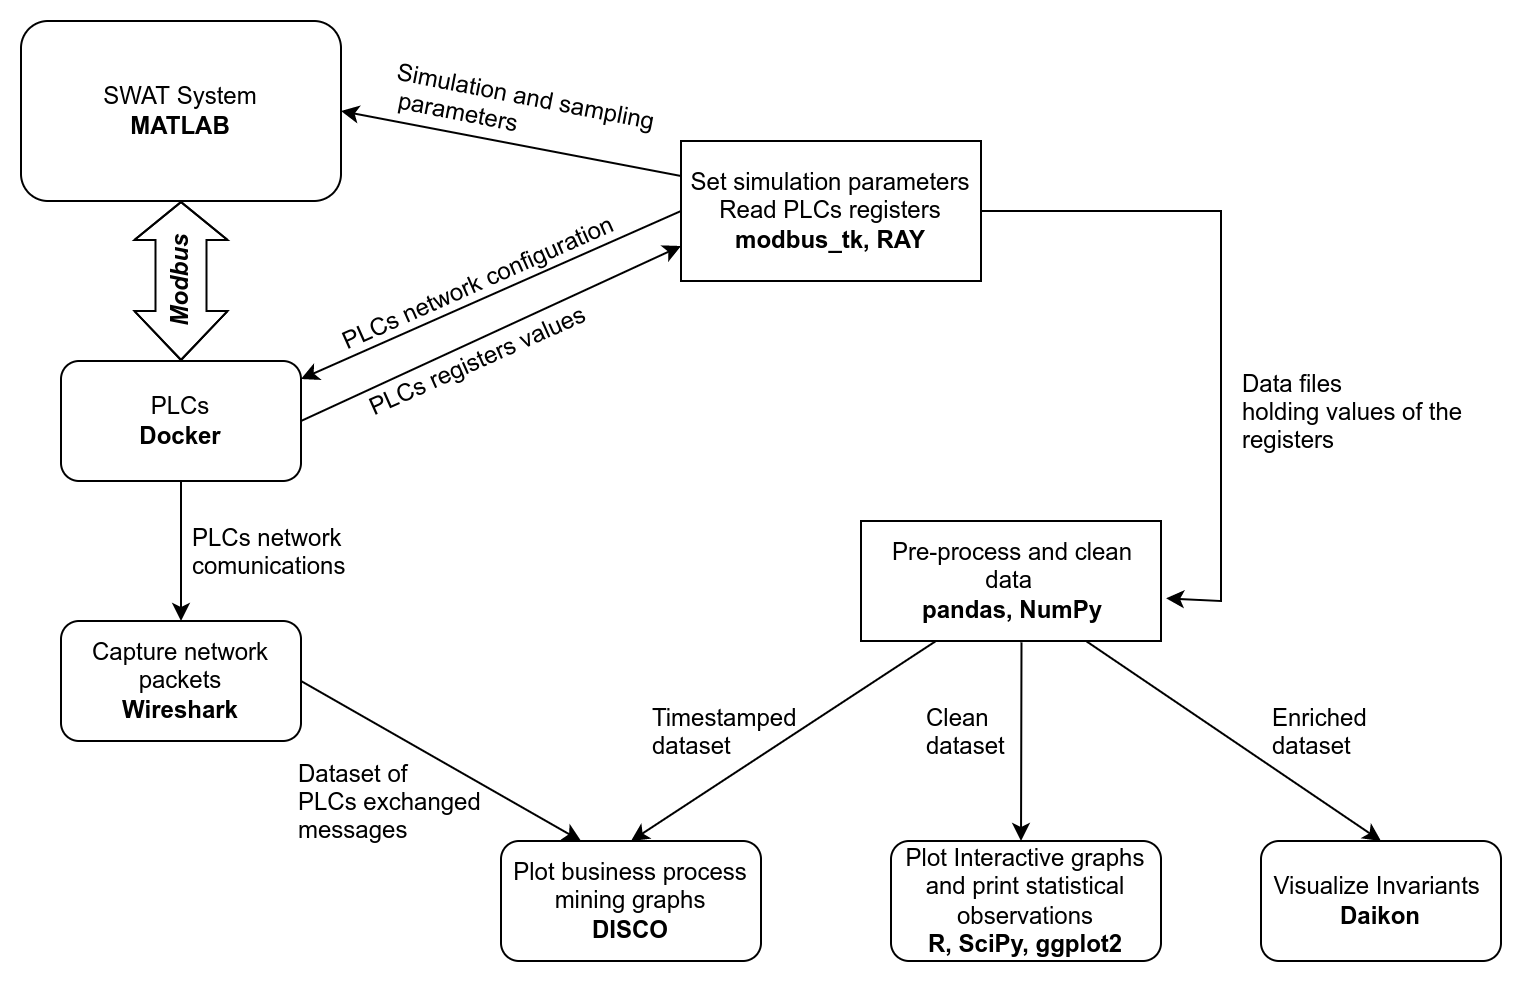
\includegraphics[scale=0.23]{chap3/ceccato_flowchart.png}
	\caption{Overview}
	\label{fig:ceccato_overview}
\end{figure}

\subsection{Testbed}
\label{subsec:ceccato_testbed}
Before describing the various phases of the methodology, let's take a look at the testbed on which this methodology will be tested. The testbed used to test this methodology is a (very) simplified version of the iTrust SWaT system \cite{swat_home} implemented by Lanotte et al. \cite{lanotte_et_al}: in Figure 3.2 we can see a graphical representation of the testbed. This simplified version consists of three stages, each controlled by a dedicated PLC: 

\begin{figure}[ht]
	\centering
	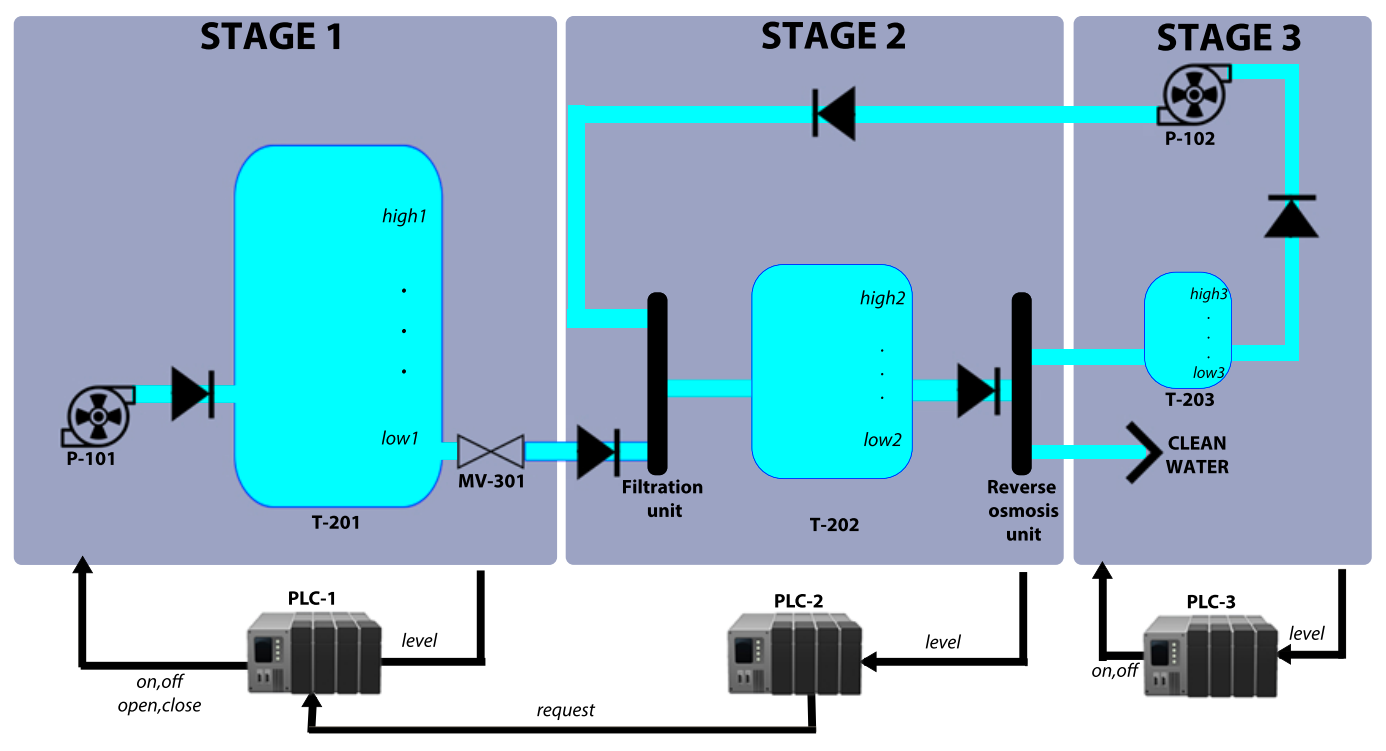
\includegraphics[scale=0.27]{chap3/univr_testbed.png}
	\caption{The simplified SWaT system used for running Ceccato et al. methodology}
	\label{fig:univr_testbed}
\end{figure}

\bigskip
\begin{description}
	\item[\textit{Stage 1}] At the first stage, a \textbf{tank} with a capacity of 80 gallons (identified by the code T-201) is filled with raw water by the P-101 pump: the MV-301 valve (where MV stands for \textit{motorized valve}), also connected to the T-201 tank, flushes out the water collected in the tank to send it to the second stage, first to the \textit{filtration unit} (here not identified by any sensor) and from there to a \textbf{second tank}, identified by the code T-202 and with a capacity of 20 gallons.
	
	\item[\textit{Stage 2}] At the second stage, water contained in T-202 flows into the \textit{reverse osmosit unit} (RO, which in this case also acts as a valve, extracting water continuously: however, it is not identified as a pump) to reduce organic impurities in the same water. The water then flows from the \textit{RO unit} to the third and last stage.
	
	\item[\textit{Stage 3}] At the third stage, the water from the \textit{RO unit} is divided according to whether standards are met: if the water is clean it will be fed into the distribution system, otherwise it will go to a \textit{backwash tank}, identified by code T-203 and a capacity of one gallon. The water in this tank will then be pumped back to the stage 2 \textit{filtration unit} through pump P-102.
\end{description}

\bigskip
As mentioned, each stage corresponds to a PLC that controls it, PLC1, PLC2 and PLC3, respectively. Let us briefly see the behavior of each of them:

\begin{description}
	\item[\textit{PLC1}] PLC1 checks the level of tank T-201 distinguishing three cases:
	
	\begin{itemize}
		\item if T-201 reaches the \textit{low setpoint low1} (hardcoded in memory registers), pump \textbf{P-101 is opened} and valve \textbf{MV-301 is closed}, so that the tank can be filled
		
		\item if T-201 reaches \textit{high setpoint high1} (also hardcoded in the memory registers), pump \textbf{P-101 is closed}
		
		\item in intermediate cases, \textbf{PLC1 waits for request from PLC2} to open/close valve MV-301: if a request to open the valve MV-301 arrives, water will flow from T-201 to T-202, otherwise the valve is closed. In both situations, pump P-101 remains closed 
	\end{itemize}

	\item[\textit{PLC2}] PLC2 monitors the level of tank T-202, behaving accordingly depending on the level of water in it. Here again there are three cases to consider:
	
	\begin{itemize}
		\item if the water level reaches the \textit{low setpoint low2} (also hardcoded in the memory registers), PLC2 sends a request to PLC1 via a Modbus channel to \textbf{open valve MV-301} in order to flow water from tank T-201 to tank T-202. The transmission channel is implemented by copying a boolean value from a memory register of PLC2 to a corresponding register of PLC1
		
		\item if the water level reaches the \textit{high setpoint high2} instead (hardcoded in the memory registers as the previous setpoints), PLC2 sends PLC1 a \textbf{close request} for valve MV-301
		
		\item In intermediate cases, the valve remains open (closed) while the tank is filling (emptying)
	\end{itemize}
	
	\item[\textit{PLC3}] PLC3 monitors the level of the T-203 backwash tank, behaving accordingly. Here there are only two cases to consider: if the tank reaches the \textit{low setpoint low3}, pump \textbf{P103 is set to off}, so that the backwash tank can be filled: otherwise, if the \textit{high setpoint high3} is reached, pump \textbf{P103 is opened} and the entire content of the backwash tank pumped back to the filter unit of T-202.
	 
\end{description} 

\subsection{Scanning of the System and Data Pre-processing}
\label{subsec:ceccato_scan}
\paragraph{Scanning tool}
The Ceccato et al. scanning tool is closely derived from a project I did \cite{ns_proj} for the "\textit{Network Security}" and "\textit{Cyber Security for IoT}" courses taught by Professors Massimo Merro and Mariano Ceccato, respectively, in the 2020/21 academic year. The original project involved, in its first part, the recognition within a network of potential PLCs listening on the standard Modbus TCP port 502 using the Nmap module for Python, obtaining the corresponding IP addresses: then a (sequential) scan of a given range of the memory registers of the found PLCs was performed to collect the register data. The data thus collected were saved to a file in \textit{JavaScript Object Notation} (JSON) format for later use in the second part of my project.

\bigskip
The scanning tool by Ceccato et. al works in a similar way, but extends what I originally did by trying to discover other ports on which the Modbus protocol might be listening (since in many realities Modbus runs on different ports than the standard one, according to the concept of \textit{security by obscurity}) and, most importantly, by \textbf{parallelizing and distributing the scan} of PLC memory registers through the Ray module \cite{ray}, specifying moreover the desired granularity of the capture. An example of raw data capture can be seen at Listing \ref{lst:raw_registers_capture}:

\begin{lstlisting}[language=Python, numbers=none, caption=Example of registers capture, label=lst:raw_registers_capture]	
	"127.0.0.1/8502/2022-05-03 12_10_00.591": {
		"DiscreteInputRegisters": {"%IX0.0": "0"},
		"InputRegisters": {"%IW0": "53"},
		"HoldingOutputRegisters": {"%QW0": "0"},
		"MemoryRegisters": {"%MW0": "40","%MW1": "80"},
		"Coils": {"%QX0.0": "0"}}
\end{lstlisting}

The captured data includes PLC's IP address, Modbus port and timestamp (first line), type and name of registers with their values read from the scan (subsequent lines).

\bigskip
The tool furthermore offers the possibility, in parallel to the memory registers scan, of \textbf{sniffing network traffic} related to the Modbus protocol using the \textit{Man in the Middle} (MitM) technique on the supervisory control network using a Python wrapper for tshark/Wireshark \cite{tshark} \cite{wireshark}. An example of raw data obtained with this sniffing can be seen in Listing \ref{lst:raw_network_capture}:

\begin{lstlisting}[language=Python, numbers=none, caption=Example of raw network capture, label=lst:raw_network_capture]	
	Time,Source,Destination,Protocol,Length,Function Code,Destination Port,Source Port,Data,Frame length on the wire,Bit Value,Request Frame,Reference Number,Info
	2022-05-03 11:43:58.158,IP_PLC1,IP_PLC2,Modbus/TCP,76,Read Coils,46106,502,,76,TRUE,25,,"Response: Trans: 62; Unit: 1, Func: 1: Read Coils"
\end{lstlisting}

\paragraph{Data Pre-processing} 
The data collected by scanning the memory registers of the PLCs are then reprocessed by a Python script and converted in order to create a distinct raw dataset in \textit{Comma Separated Value} format (CSV) for each PLC, containing the memory register values associated with the corresponding controller registers. These datasets are reprocessed again through the Python modules for \textbf{pandas} \cite{pandas} and \textbf{NumPy} \cite{numpy} by another script to first perform a \textbf{data cleanup}, removing all those memory registers that do not take values and are therefore useless within the system, \textbf{merged} into a single dataset, and finally \textbf{enriched} with additional data\footnote{Not all additional data are calculated and entered automatically by the tool: some are manually inserted.}.

\bigskip
This process leads to the creation of two copies of the full dataset: one enriched with the additional data, but not timestamped, which will be used for the invariant analysis; the other unenriched, but timestamped, which will be used for business process mining.

\subsection{Graphs and Statistical Analysis}
\label{subsec:ceccato_graphanalysis}
The paper mentions the presence of a \textit{mild graph analysis}, performed with \textbf{R} \cite{r-project} at the time of data gathering to find any uncovered patterns, trends and identify measurements and/or actuator commands through the analysis of registers holding mutable values. 

\bigskip
There is actually no trace of this within the tool: \textit{graph analysis} and \textit{statistical analysis} of the data contained in the PLC memory registers are instead performed using the \textbf{matplotlib libraries} and statistical algorithms made available by the \textbf{SciPy libraries} \cite{scipy}, through two separate Python scripts (see Figure \ref{fig:ceccato_graphs}).

\begin{figure}[ht]
	\centering
	\begin{subfigure}{0.48\textwidth}
		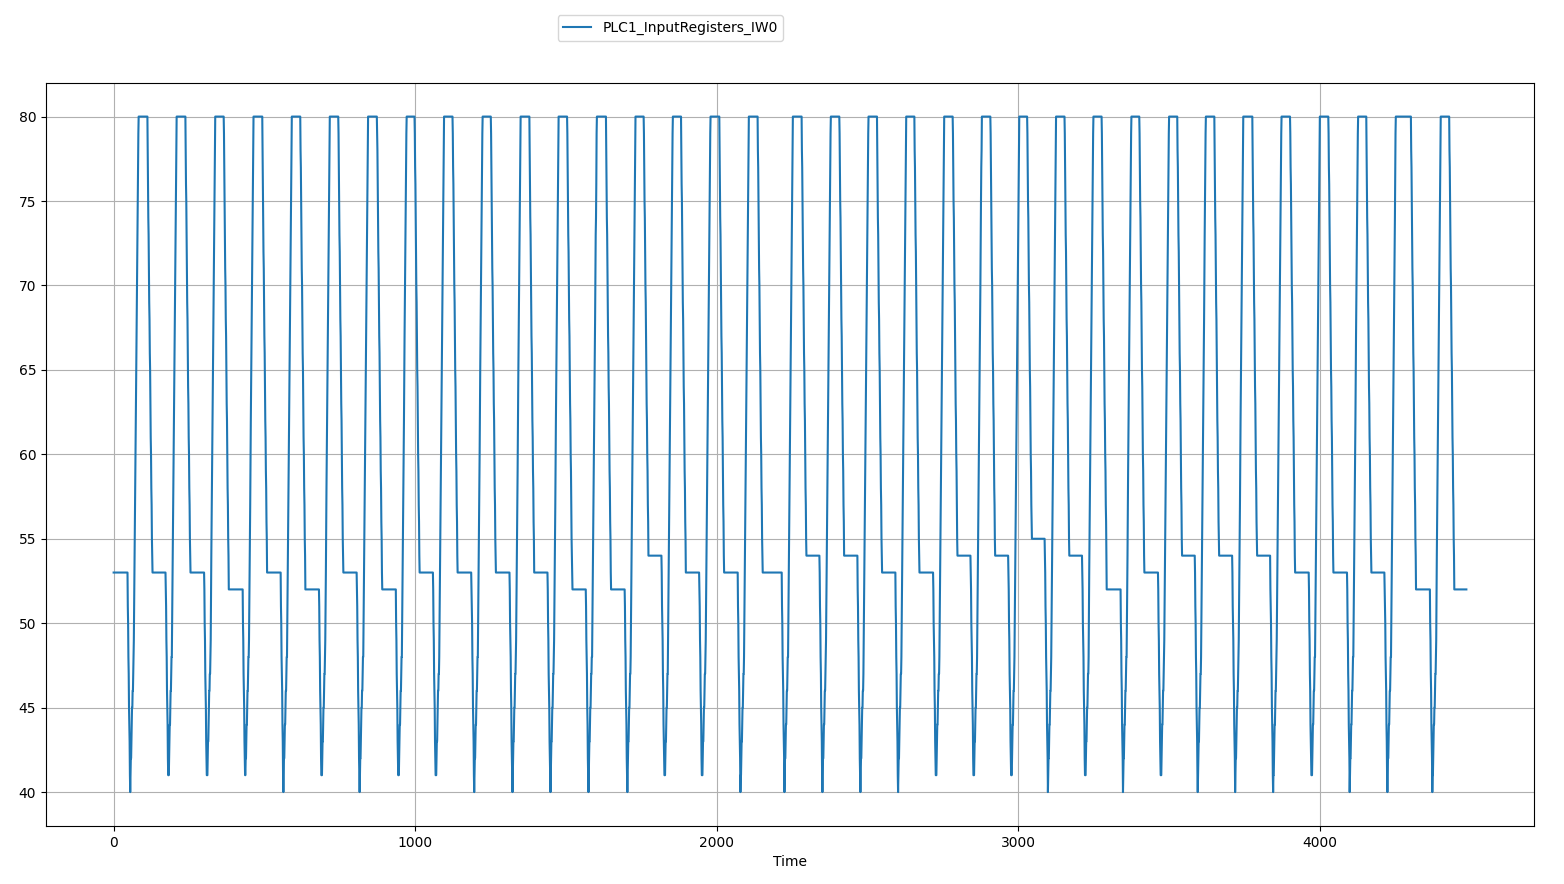
\includegraphics[width=\textwidth]{chap3/chartPlot_ceccato.png}
		\caption{Chart plot for\\ \textnormal{\texttt{PLC1\_InputRegisters\_IW01}} register}
		\label{subfig:chart_plot_ceccato}
	\end{subfigure}
	\hfill
	\begin{subfigure}{0.48\textwidth}
		\includegraphics[width=\textwidth]{chap3/histPlot_ceccato.png}
		\caption{Histogram plot for\\ \textnormal{\texttt{PLC1\_InputRegisters\_IW01}} register}
		\label{subfig:hist_plot_ceccato}
	\end{subfigure}
	\caption{Output graphs from graph analysis}
	\label{fig:ceccato_graphs}
\end{figure}

The first script plots the charts, one at the time, of certain registers entered by the user from the command line, plots in which one can see the trend of the data and get a first basic idea of what that particular register contains (a measurement, an actuation, a hardcoded setpoint, ...) and possibly the trend; the second script, instead, shows \textbf{a histogram and statistical informations} about the register entered as command-line input. These informations include:

\begin{itemize}
	\item the mean, median, standard deviation, maximum value and minimum value
	
	\item two tests for the statistical distribution: \textit{Chi-squared} test for uniformity and \textit{Shapiro-Wilk} test for normality, as shown in Listing \ref{lst:stats_anal}:

\end{itemize}

\begin{lstlisting}[language=Python,numbers=none,caption={Statistical data for \textnormal{\texttt{PLC1\_InputRegisters\_IW0}} register},label=lst:stats_anal]
	Chi-squared test for uniformity
	Distance      pvalue    Uniform?
	12488.340   0.00000000    NO    
	
	Shapiro-Wilk test for normality
	Test statistic    pvalue    Normal? 
	0.844   0.00000000    NO    
	
	Stats of PLC1_InputRegisters_IW0
	Sample mean = 60.8881; Stddev = 13.0164; max = 80; min = 40 for 4488 values
\end{lstlisting}

\subsection{Invariants Inference and Analysis}
\label{subsec:ceccato_invariants}
For invariant analysis Ceccato et al. rely on \textbf{Daikon} \cite{daikon_site}, a framework to \textbf{dynamically detect likely invariants} within a program. An \textit{invariant} is a property that holds at one or more points in a program, properties that are not normally made explicit in the code, but within assert statements, documentation and formal specifications: invariants are useful in understanding the behavior of a program (in our case, of the cyber physical system).

Daikon uses \textit{machine learning} techniques applied to arbitrary data with the possibility of setting custom conditions for analysis by using a specific file \cite{daikon_spinfo} with a \textit{.spinfo} extension (see Listing \ref{lst:spinfo}). The framework is designed to find the invariants of a program, with various supported programming languages, starting from the direct execution of the program itself or passing as input the execution run (typically a file in CSV format): the authors of the paper tried to apply it by analogy also to the execution runs of a cyber physical system, to extract the invariants of this system.

\begin{lstlisting}[language=Python,numbers=none,caption={Generic example of a .spinfo file for customizing rules in Daikon},label=lst:spinfo]
	PPT_NAME aprogram.point:::POINT
	VAR1 > VAR2
	VAR1 == VAR3 && VAR1 != VAR4
\end{lstlisting}

Therefore, Daikon is fed with the no-timestamp enriched dataset obtained in the pre-processing phase (in the paper, the timestamped dataset is erroneously mentioned as input): a simple bash script launches Daikon (optionally specifying the desired condition for analysis in the \textit{.spinfo} file), which output is simply redirected to a text file containing the general invariants of the system (i.e., valid regardless of any custom condition specified), those generated based on the custom condition in the \textit{.spinfo} file, and those generated based on the negation of the condition. When the analysis is finished, the user is asked to enter the name of a registry to view its related invariants.\newline \newline
Some examples of invariants derived from the enriched dataset may be:

\begin{itemize}
	\item measurements bounded by some setpoint
	
	\item Actuators state changes occourred in the proximity of setpoints or, vice versa, proximity of setpoints upon the occurrence of a regular actuator state change
	
	\item state invariants of some actuator correspond to a specific trend in the evolution of the measurement (ascending, descending, or stable) or, vice versa, the measurement trend corresponds to a specific state invariant of some actuator
\end{itemize}
\vfill

\subsection{Businness Process Mining and Analysis}
\label{subsec:ceccato_businessprocess}
\textit{Process mining} is the analysis of operational processes based on the event log \cite{process_mining_def}: the aim of this analysis is to \textbf{extract useful informations} from the event data to \textbf{reconstruct and understand the behavior} of the business process and how it was actually performed.

\bigskip
Process mining for the system under consideration starts from the event logs obtained from scanning the memory registers of the PLCs and sniffing the network communications related to the Modbus protocol, described in Subsection \ref{subsec:ceccato_scan} and representing the \textit{execution trace} of the system: through a Java program, information is extracted and combined from these event logs, and the result saved in a CSV format file.

This file is fed to \textbf{Disco} \cite{disco}, a commercial process mining tool, which generates an \textit{activity diagram} similar to UML Activity Diagram and whose nodes represent the activities while the edges represent the relations between these activities: in Figure \ref{fig:disco_example} we can see an example of this diagram referred to PLC2 of the testbed.

\begin{figure}[ht]
	\centering
	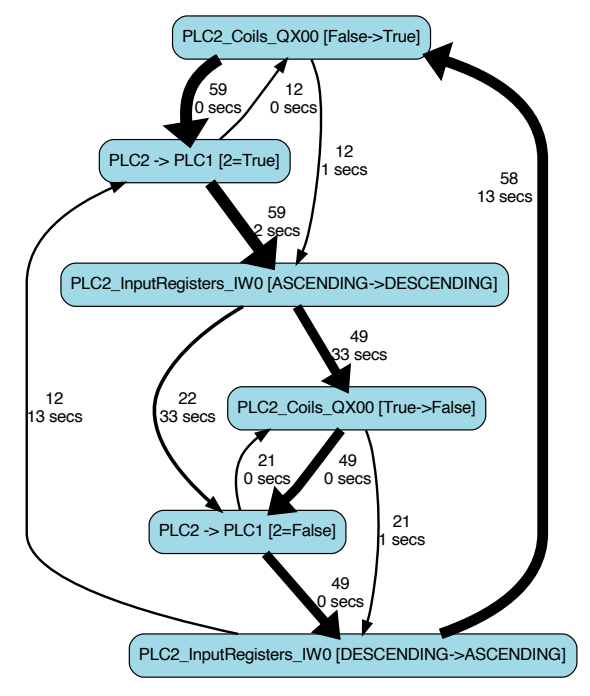
\includegraphics[scale=0.30]{chap3/disco_example.png}
	\caption{An example of Disco generated activity diagram for PLC2}
	\label{fig:disco_example}
\end{figure}

The \textit{business process} obtained in this way provides an \textbf{overview of the system} and makes it possible to \textbf{make conjectures} about its behavior, particularly between changes in actuator state and measurement trends (i.e., a given change in state of some actuators corresponds to a specific measurement trend and vice versa), and with the possibility of \textbf{establishing causality} between Modbus communications and state changes within the physical system.

\subsection{Application}
\label{subsec:ceccato_application}
In this section we will see how the black box analysis presented above in its various phases is applied in practice, using the testbed described in Subsection \ref{subsec:ceccato_testbed}.
The methodology supports a \textbf{\textit{top-down} approach}: that is, we start with an overview of the industrial process and then gradually refine our understanding of the process by descending to a higher and higher level of detail based on the results of the previous analyses and focusing on the most interesting parts of the system for further in-depth analysis.

\paragraph{Data Collection and Pre-processing} 
According to what is described in the paper, the data gathering process lasted six hours, with a granularity of one data point per second (a full system cycle takes approximately 30 minutes). Each datapoint consists of 168 attributes (55 registers plus a special register concerning the tank slope of each PLC) after the enrichment. In addition, IP addresses are automatically replaced by an abstract name identified by the prefix PLC followed by a progressive integer (PLC1, PLC2, PLC3), in order to make reading easier.

\paragraph{Graphs and Statistical Analysis}
It is unclear from the paper where exactly the information that follows was derived (graph analysis? Statistical analysis? Human reading of the dataset?), however, three properties about the contents of the registers were discovered: 

\begin{description}
	\item[\colorbox{backcolourtext}{\textnormal{\textit{Property 1:}}}] \texttt{PLC1\_MemoryRegisters\_MW0},  \texttt{PLC1\_MemoryRegisters\_MW1}, \\ \texttt{PLC2\_MemoryRegisters\_MW0},  \texttt{PLC2\_MemoryRegisters\_MW1}, \\ 
	\texttt{PLC3\_MemoryRegisters\_MW0} and 
	\texttt{PLC3\_MemoryRegisters\_MW1}
 
	registers contain constant integer values (40, 80, 10, 20, 0, 10 respectively)\footnote{From my tests on the original tool and dataset, the \texttt{PLC3\_MemoryRegisters\_MW0} register is deleted during the \textit{pre-processing} phase, as it is recognized as an unused register because of the constant value "0" it takes on. This leads me to assume that the properties are derived from a human read of the dataset prior to the \textit{pre-processing} phase.}. We may speculate that they may be (relative) hardcoded \textbf{setpoints}.
	
	\item[\colorbox{backcolourtext}{\textnormal{\textit{Property 2:}}}] \texttt{PLC1\_Coils\_QX01}, \texttt{PLC1\_Coils\_QX02}, \texttt{PLC2\_Coils\_QX01}, \\ \texttt{PLC2\_Coils\_QX02}, \texttt{PLC3\_Coils\_QX01} and \texttt{PLC3\_Coils\_QX03} contain mutable binary (Boolean) values.
	We can assume that these registers can be associated with the \textbf{actuators} of the system.
	
	\item[\colorbox{backcolourtext}{\textnormal{\textit{Property 3:}}}] \texttt{PLC1\_InputRegisters\_IW0},
	\texttt{PLC2\_InputRegisters\_IW0} and \\ \texttt{PLC3\_InputRegisters\_IW0} registers contain mutable values.
\end{description}

\textit{Property 3} suggests that those registers might contain \textbf{values related to measurements}: it is therefore necessary to investigate further to see if the conjecture (referred to as \textit{Conjecture 1} in the paper) is correct.

\begin{figure}[ht]
	\centering
	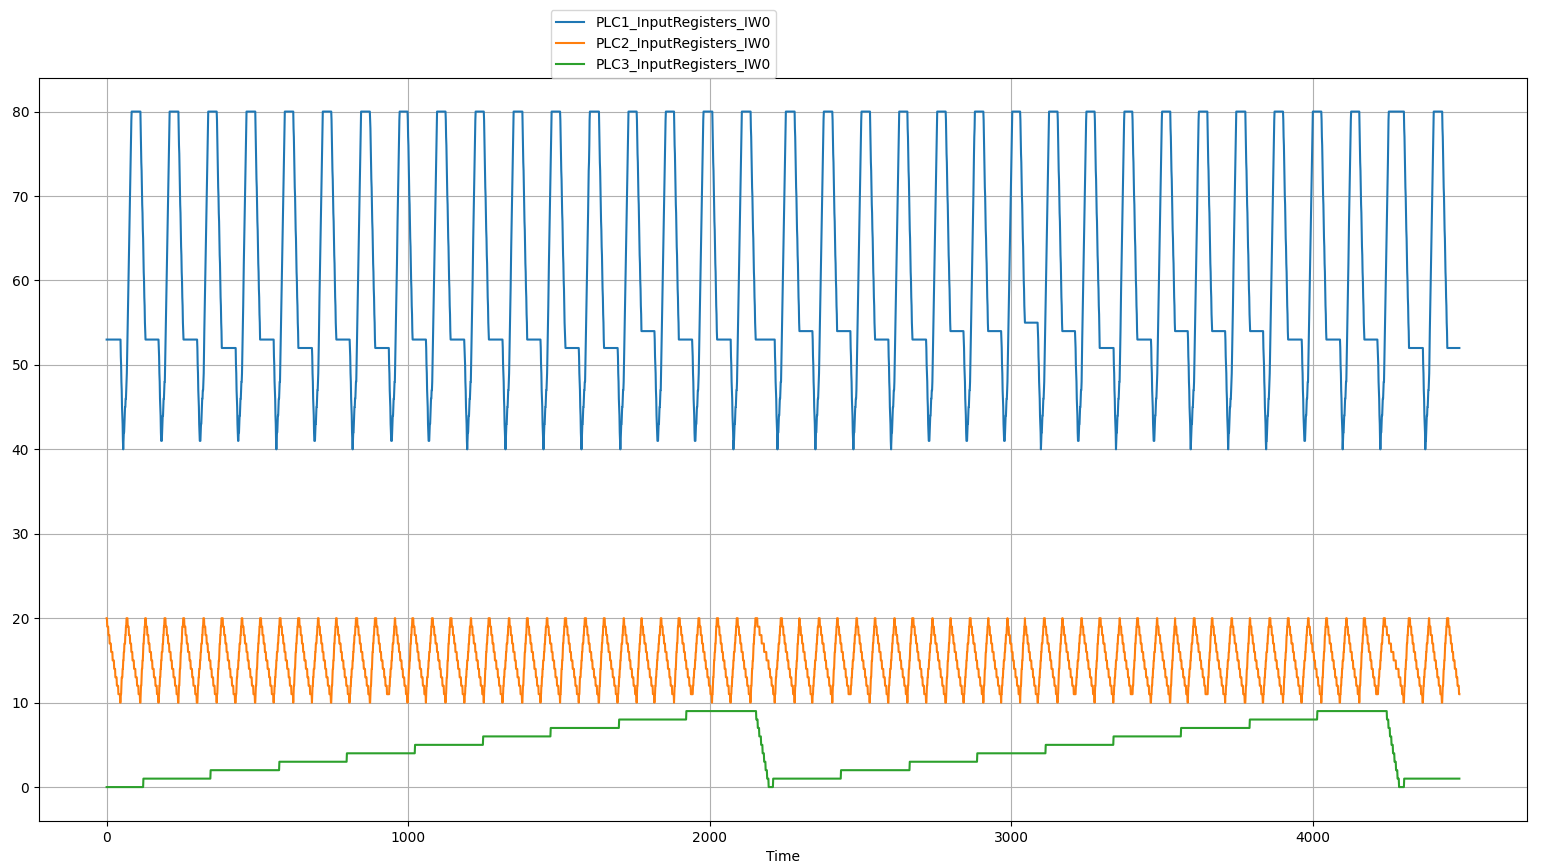
\includegraphics[scale=0.30]{chap3/graph_analysis_prop3_ceccato.png}
	\caption{Execution traces of InputRegisters\_IW0 on the three PLCs}
	\label{fig:graph_analysis_prop3}
\end{figure}

The graph analysis of the \texttt{InputRegisters\_IW0} registers of the three PLCs (summarized in Figure \ref{fig:graph_analysis_prop3} with a single plot) not only seems to confirm the conjecture, but also allows the measurements to be correlated with the contents of the \texttt{MemoryRegisters\_MW0} and \texttt{MemoryRegisters\_MW1} registers to the measurements, which represent the \textbf{relative setpoints of the measurements}.\\
Hence, we have \textit{Conjecture 2} described in the paper referring to the relative setpoints:\newline \newline
\colorbox{backcolourtext}{\emph{Conjecture 2:}} 

	- 40 and 80 are the relative setpoints for \texttt{PLC1\_InputRegisters\_IW0}
	
	- 10 and 20 are the relative setpoints for \texttt{PLC2\_InputRegisters\_IW0}
	
	- 0 and 9 are the relative setpoints for \texttt{PLC3\_InputRegisters\_IW0} 

\bigskip
Further confirmation of this conjecture may come from statistical analysis. Indeed, in the example in Listing 3.1, some statistical data are given for the register \texttt{PLC1\_InputRegisters\_IW0}, including the maximum value and the minimum value: these values are, in fact, 80 and 40 respectively.

\paragraph{Business Process Mining and Analysis}
With Business Process Mining, the authors aim to \textbf{visualize and highlight relevant system behaviors} by relating PLC states and Modbus commands.

\bigskip
Through analysis of the activity diagrams shown in Figure \ref{fig:business_process_cecccato}, drawn through Disco, we derive the following properties and conjectures:

\begin{description}
	\item[\colorbox{backcolourtext}{\textnormal{\textit{Property 4:}}}] PLC2 sends messages to PLC1 (see Figure \ref{subfig:pm_plc2}) which are recorded to \texttt{PLC1\_Coils\_QX02}.
	
	\item[\colorbox{backcolourtext}{\textnormal{\textit{Conjecture 3:}}}] \texttt{PLC2\_Coils\_QX00} determines the trend in tank T-202 (Figure \ref{subfig:pm_plc2}). \newline
	When this register is set to \textit{True}, the input register \texttt{PLC2\_InputRegisters\_IW0} related to the tank controlled by PLC2 starts an \textbf{ascending trend}; vice versa, when the coil register is set to \textit{False}, the input register starts a \textbf{descending trend}.
	
	\item[\colorbox{backcolourtext}{\textnormal{\textit{Conjecture 4:}}}] If \texttt{PLC1\_Coils\_QX00} change his value to True, trend in tank T-201, related to \texttt{PLC1\_InputRegisters\_IW0} and controlled by PLC1, become \textbf{ascending} (see Figure \ref{subfig:pm_plc1})
	
\end{description}

\begin{figure}[H]
	\centering
	\begin{subfigure}{0.7\textwidth}
		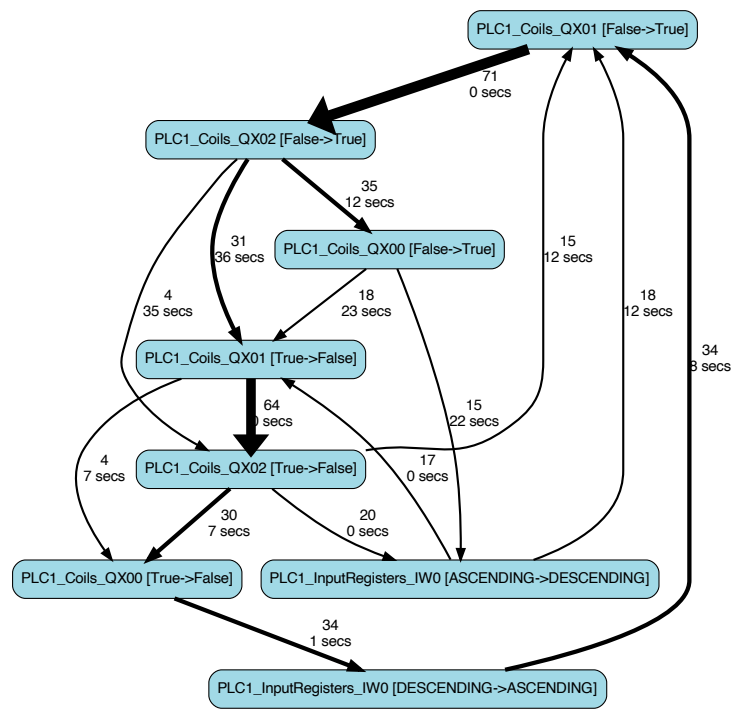
\includegraphics[width=\textwidth]{chap3/disco_plc1.png}
		\caption{States in PLC1}
		\label{subfig:pm_plc1}
	\end{subfigure}
	\hfill
	\begin{subfigure}{0.48\textwidth}
		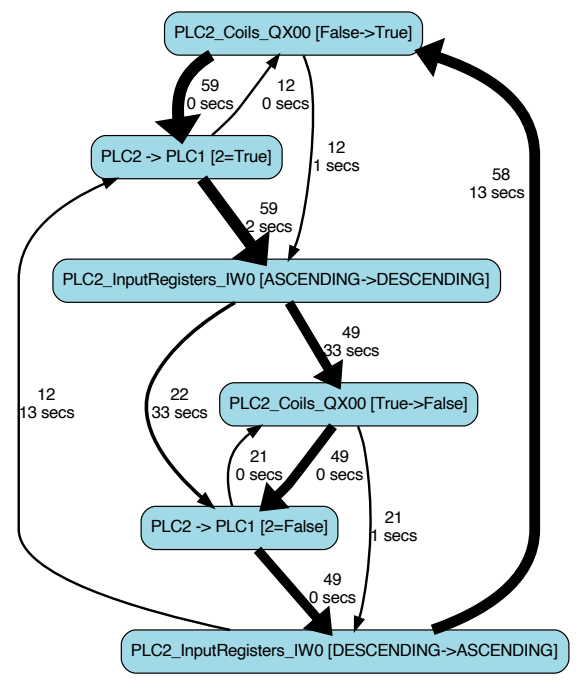
\includegraphics[width=\textwidth]{chap3/disco_plc2.png}
		\caption{States and Modbus command in PLC2}
		\label{subfig:pm_plc2}
	\end{subfigure}
	\hfill
	\begin{subfigure}{0.48\textwidth}
		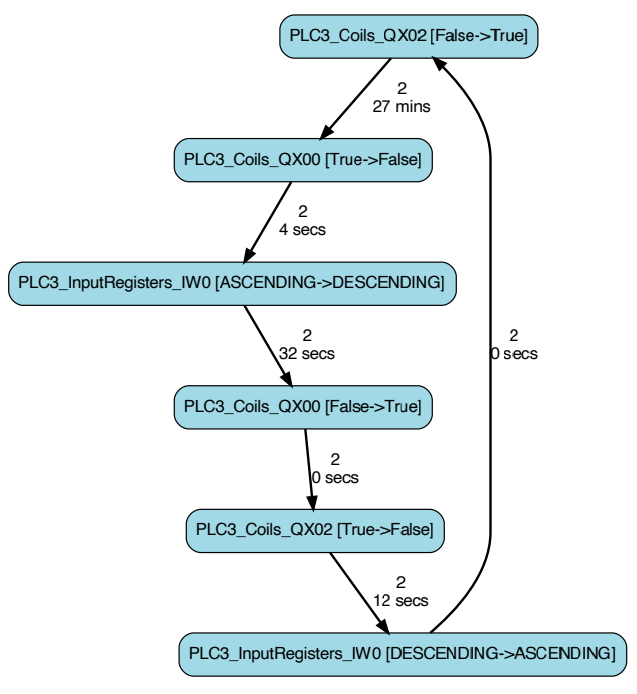
\includegraphics[width=\textwidth]{chap3/disco_plc3.png}
		\caption{States in PLC3}
		\label{subfig:pm_plc3}
	\end{subfigure}
	\caption{Business process with states and Modbus commands for the three PLCs}
	\label{fig:business_process_cecccato}
\end{figure}
\pagebreak

\begin{description}
	\item[\colorbox{backcolourtext}{\textnormal{\textit{Conjecture 5:}}}] \texttt{PLC3\_Coils\_QX00} starts a \textbf{decreasing trend} in tank T-203, related to \texttt{PLC3\_InputRegisters\_IW0} and controlled by PLC3, whereas \texttt{PLC3\_Coils\_QX02} starts an \textbf{increasing trend} on the tank (see Figure \ref{subfig:pm_plc3})
\end{description}

\paragraph{Invariants Inference and Analysis}
The last phase of the analysis of the example industrial system is invariant analysis, performed through Daikon framework. At this stage, an attempt will be made to confirm what has been seen previously and to derive new properties of the system based on the results of the Daikon analysis.

\bigskip
To get gradually more and more accurate results, the authors presumably performed more than one analysis with Daikon, including certain rules within the \textit{splitter information file} (see Section \ref{subsec:ceccato_invariants} and Listing \ref{lst:spinfo}) based on specific conditions placed on the measurements, for example, the level of water contained in a tank. Given moreover the massive amount of invariants generated by Daikon's output, it is not easy to identify and correlate those that are actually useful for analysis: this must be done manually.

\bigskip
However, it was possible to have confirmation of the conjectures made in the previous stages of the analysis: starting with the setpoints, analyzing the output of the invariants returned by Daikon\footnote{The invariants shown here are a manual summary and derivation of those actually returned in output by Daikon. I will discuss this more in Section \ref{subsec:ceccato_limitations}} reveals that \newline \newline
\small\texttt{PLC1\_InputRegisters\_IW0 >= PLC1\_MemoryRegisters\_MW0 == 40.0}\\
\texttt{PLC1\_InputRegisters\_IW0 <= PLC1\_MemoryRegisters\_MW1 == 80.0}\\
\texttt{PLC2\_InputRegisters\_IW0 >= PLC2\_MemoryRegisters\_MW0 == 10.0}\\
\texttt{PLC2\_InputRegisters\_IW0 <= PLC2\_MemoryRegisters\_MW1 == 20.0}\\
\texttt{PLC3\_InputRegisters\_IW0 >= PLC3\_MemoryRegisters\_MW0 == 0.0}\\
\texttt{PLC3\_InputRegisters\_IW0 <= PLC3\_MemoryRegisters\_MW1 == 9.0} \newline \newline
\normalsize i.e., that the \texttt{MemoryRegisters\_MW0} and \texttt{MemoryRegisters\_MW1} registers of each PLC contain the \textbf{absolute minimum and maximum setpoints}, respectively (\textit{Property 5}).

\bigskip
There is also a confirmation regarding \textit{Property 4}: from the computed invariants it can be seen that \newline \newline
\small\texttt{PLC1\_Coils\_QX01 == PLC1\_Coils\_QX02 == PLC2\_Coils\_QX00}\newline \newline
\normalsize and from this derive that there is a \textbf{communication channel between PLC2 and PLC1}, where the value of \texttt{PLC2\_Coils\_QX00} is copied to \texttt{PLC1\_Coils\_QX01} and \texttt{PLC1\_Coils\_QX02} (\textit{Property 6}).

\bigskip
Regarding the \textbf{relationships between actuator state changes and measurement trends}, invariant analysis yields the results summarized in the following rules:

\begin{description}
	\item[\colorbox{backcolourtext}{\normalfont\textit{Property 7:}}] Tank T-202 level \textit{increases} iif \texttt{PLC1\_Coils\_QX01 == True}. Otherwise, if \texttt{PLC1\_Coils\_QX01 == False} will be \textit{non-increasing}.
\end{description}
	This is because if the coil is \textit{True} the condition \newline \scriptsize\texttt{PLC2\_InputRegisters\_IW0 == PLC2\_MemoryRegisters\_MW0 == 20.0 \&\& PLC2\_slope > 0} \newline \normalsize is verified. 
	On the opposite hand, if the coil is \textit{False}, the condition \newline \scriptsize\texttt{PLC2\_InputRegisters\_IW0 == PLC2\_MemoryRegisters\_MW0 == 20.0 \&\& PLC2\_slope <= 0}  \normalsize is verified. The \textit{slope} is an auxiliary attribute indicating the trend of the measurement: increasing if > 0, decreasing if < 0, stable otherwise.

\begin{description}
	\item[\colorbox{backcolourtext}{\normalfont\textit{Property 8:}}] Tank T-201 level \textit{increases} iif \texttt{PLC1\_Coils\_QX00 == True}. On the other hand, if \texttt{PLC1\_Coils\_QX00 == False} and if \texttt{PLC1\_Coils\_QX01 == True} the level will be \textit{non-decreasing}.
	
	\item[\colorbox{backcolourtext}{\normalfont\textit{Property 9:}}] Tank T-203 level \textit{decreases} iif \texttt{PLC3\_Coils\_QX00 == True}. It will be \textit{non-decreasing} if \texttt{PLC1\_Coils\_QX00 == False}.
\end{description}

The last two properties concern the \textbf{relationship between actuator state changes and the setpoints}: it is intended to check what happens to the actuators when the water level reaches one of these setpoints. From the analysis of the relevant invariants, the following properties are derived:

\begin{description}
	\item[\colorbox{backcolourtext}{\normalfont\textit{Property 10:}}] Tank T-201 reaches the upper absolute setpoint when\\ \texttt{PLC1\_Coils\_QX00} changes its state from \textit{True} to \textit{False}. If the coil changes from \textit{False} to \textit{True}, the tank reaches its absolute lower setpoint.
	
	\item[\colorbox{backcolourtext}{\normalfont\textit{Property 11:}}]
	Tank T-203 reaches the upper absolute setpoint when\\ \texttt{PLC3\_Coils\_QX00} changes its state from \textit{True} to \textit{False}. If the coil changes from \textit{False} to \textit{True}, the tank reaches its absolute lower setpoint.	 
\end{description}

\subsection{Limitations}
\label{subsec:ceccato_limitations}
The methodology proposed by Ceccato et al. is certainly valid and offers a good starting point for approaching the reverse engineering of an industrial control system from the attacker's perspective, while also providing a tool to perform this task.

\bigskip
The limitations of this approach, however, all lie in the tool mentioned above and also in the testbed described in Section \ref{subsec:ceccato_testbed}. In this section I will explain which are the criticisms of each phase, while in Chapter 4 I will formulate proposals to improve and make this methodology more efficient.

\paragraph{General Criticism}
\label{par:limit_ceccato_general}
The general critical aspects of the application of this approach are many: the primary one concerns the fact that the proposed tool seems to be built specifically for the testbed used and that it is not applicable to other contexts, even to the same type of industrial control system (water treatment systems, in this case). 

\bigskip
What severely limits the analysis performed with the tool implemented by Ceccato et al. is the use of \textit{ad hoc} solutions and \textit{a posteriori} interventions done manually on the datasets after the data gathering process: I will discuss this last aspect in more detail later.\newline
Moreover, there is the presence of many \textit{hardcoded} variables and conditions within the scripts: this makes the system unconfigurable and unable to properly perform the various stages of the analysis as errors can occur due to incorrect data and mismatches with the system under analysis.

Having considered, furthermore, only the Modbus protocol for network communications between the PLCs is another major limiting factor and does not help the methodology to be adaptable to different systems communicating with different protocols (sometimes even multiple ones on the same system). 

\bigskip
Let us now look at the limitations and critical aspects of each phase.

\paragraph{Testbed}
\label{par:limit_ceccato_testbed}
The testbed environment used by Ceccato et. al is entirely simulated, from the physical system to the control system. The PLCs were built with \textbf{OpenPLC} \cite{openplc} in a Docker environment \cite{docker}, while the physics part was built through \textbf{Simulink} \cite{simulink}.

\bigskip
OpenPLC is an open source cross-platform software that simulates the hardware and software functionality of a physical PLC and also offers a complete editor for PLC program development with support for all standard languages: \textit{Ladder Logic} (LD), \textit{Function Block Diagram} (FBD), \textit{Instruction List} (IL), \textit{Structured Text} (ST), and \textit{Sequential Function Chart} (SFC).\newline
It is for sure an excellent choice for creating a zero-cost industrial or home automation and \textit{Internet of Things} (IoT) system that is easy to manage via a dedicated, comprehensive and functional web interface. In spite of these undoubted merits, however, there are (at the moment) \textbf{very few supported protocols}: the main one and also referred to in the official documentation is \textbf{Modbus}, while the other protocol is DNP3.

\bigskip
The biggest problem with the testbed, however, is not with the controller part, but with the \textbf{physical part}: first of all, it must be said that although this is something purely demonstrative even though it is fully functional, the implemented Simulink model is really \textbf{oversimplified} compared to the iTrust SWaT system, which itself is a scaled-down version of a real water treatment plant. In fact, in the entire system there are only three actuators, two of which are connected to the same tank and controlled by the same PLC, and sensors related only to the water level in the system's tanks: in a real system there are many more \textit{field devices}, which can monitor and control other aspects of the system beyond the mere contents of the tanks. Consider, for example, measuring and controlling the chemicals in the water, the pressure of the liquid in the filter unit, or more simply the amount of water flow at a given point or time.\newline
All these must be considered and represent a number of additional variables that makes analysis and consequently reverse engineering of the system more difficult.

\bigskip
The second critical aspect concerns the \textbf{simulation of the physics of the liquid} inside the tanks: Simulink does not consider the fact that inside a tank that is filling (emptying) the liquid in it undergoes \textbf{fluctuations} which cause the level sensor not to see the water level constantly increasing (decreasing) or at most being stable at each point of detection. Figure \ref{fig:testbed_physics} exemplifies more clearly with an example the concept just expressed: these oscillations cause a \textbf{perturbation} in the data.\newline
This issue leads to the difficulty, on a real physical system, of \textbf{correctly calculating the trend of a measurement} by using the slope attribute: if this was obtained with a too low granularity, the trend will be oscillating between increasing and decreasing even when in reality this would be in general increasing (decreasing) or stable; on the other hand, if the slope was obtained with a too high granularity there is a loss of information and the trend may be "flattened" with respect to reality.\newline
In the present case, the slope in the Simulink model was calculated statically \textit{point-to-point}, thus with a granularity of one second: an averagely careful reader will have already guessed that this granularity is inapplicable to the real system in Figure \ref{subfig:real_physics}. As we will later see, we need to \textbf{operate on the data perturbations} to be able to obtain a suitable granularity and a correct calculation of the slope and consequently of the measurement trend.
\vfill

\pagebreak
\begin{figure}[ht]
	\centering
	\begin{subfigure}{0.9\textwidth}
		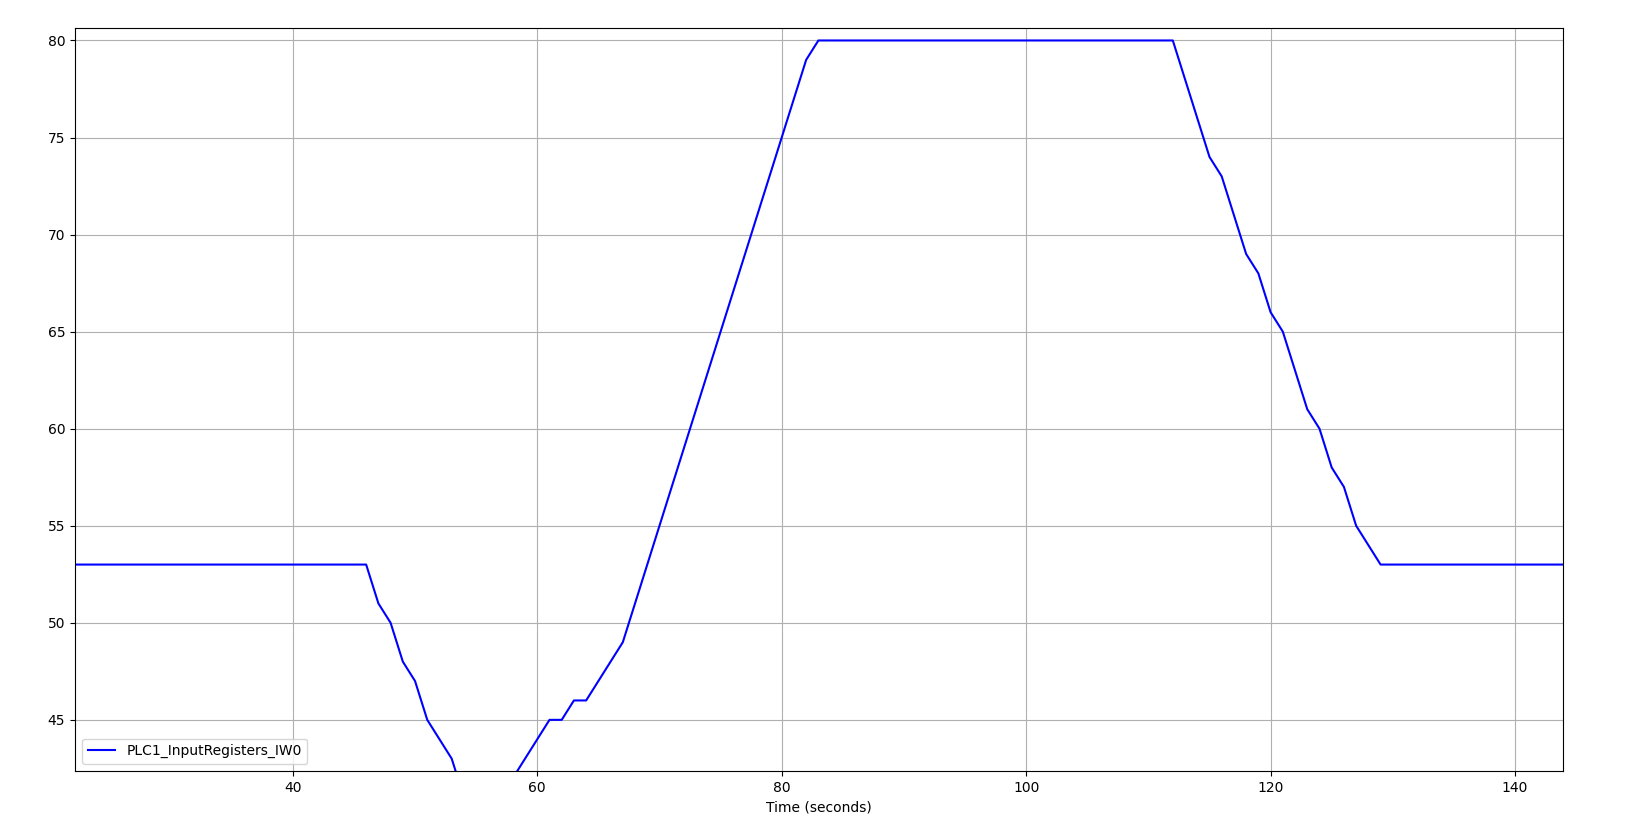
\includegraphics[width=\textwidth]{chap3/simulink_physics.png}
		\caption{}
		\label{subfig:simulink_physics}
	\end{subfigure}
	\hfill
	\begin{subfigure}{0.9\textwidth}
		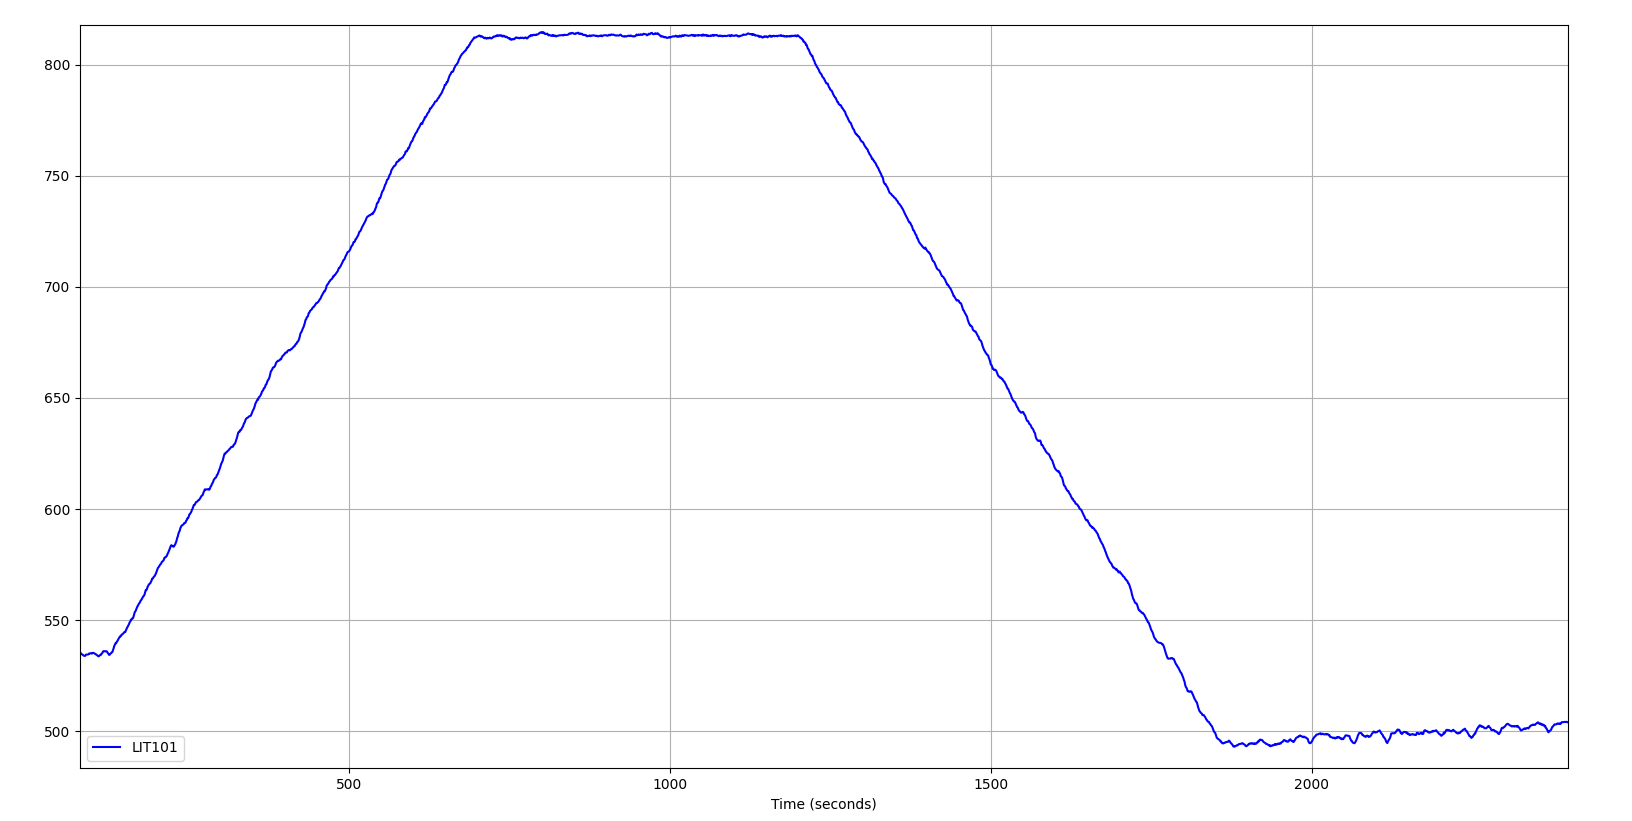
\includegraphics[width=\textwidth]{chap3/real_physics.png}
		\caption{}
		\label{subfig:real_physics}
	\end{subfigure}
	\caption{Water physics compared: simulated physics in the Simulink model (a) and physics in a real system (iTrust SWaT) (b). Fluctuations in the tank level in (b), almost completely absent in (a), can be appreciated.}
	\label{fig:testbed_physics}
\end{figure}

\paragraph{Pre-processing}
\label{par:limit_ceccato_preproc}

\paragraph{Graphs and Statistical Analysis}
\label{par:limit_ceccato_graphs}

\paragraph{Business Process Mining and Analysis}
\label{par:limit_ceccato_pm}

\paragraph{Invariants Inference and Analysis}
\label{par:limit_ceccato_invariants}

\vfill
\nolinenumbers
